\section{Tipi di controlli sulle frodi}

\begin{itemize}
\item Controlli correttivi (\emph{Corrective Controls}) \\
Risolve probemi e previeni problemi future.
\item \emph{Detecive Controls}\todo{Trova una traduzione sensata}\\ 
\item Controlli preventivi (\emph{Preventive Controls})\\
Previene le frodi.
Include:
	\begin{itemize}
	\item Risk Assessment
	\item Sviluppo di controlli interni
	\item Sicurezza fisica e informatica
	\item Autorizzazioni (Password, ecc.)
	\item Segregation of Duties
	\end{itemize}
\end{itemize}

I controlli eseguiti in maniera preventiva sono sempre meglio rispetto alle
altre tipologie di controlli.

La sicurezza fisica, come la protezione di alcuni locali all'interno
dell'azienda (per esempio una sala server) va sempre ritenuta in
considerazione, e non va trascurata.

\subsection{Tecniche per scoraggiare una frode}

L'aspetto motivazionale è molto spesso da tenere in considerazione.
Un utente che esce con un alto grado di studio potrebbe subire delle
frustrazioni se gli viene assegnato un lavoro troppo basso per il suo livello.

Altro errore da non sottovalutare è la promozione: dopo 8 anni di solito una
persona si aspetta di essere promossa.

L'esempio è anche importante: le persone nell'alta gerarchia diventano un
\textbf{role model}, ovvero i sottoposti prendono ispirazione dai dirigenti, ed è
quindi fondamentale che essi abbiano un comportamento esemplare.

Ma come si rimuove la possibilità di una frode?
\begin{itemize}
  \item \textit{Segregation of duties}.
  \item Sicurezza dei beni.
  \item Sicurezza fisica (sono presenti tornelli per accedere a determinate
aree per esempio?)
  \item \textit{Background checks} spesso eseguiti:
  \begin{itemize}
    \item Su titoli di studio
    \item Su casi penali
  \end{itemize}
\end{itemize}

\subsubsection{Segregation of Duties}

Bisogna fare in modo che il potere associato ad una certa funzione non risieda
nelle mani di una sola persona:
Esistono tre fondamenti per una corretta \textbf{segregation of duties}:
\begin{itemize}
  \item Origine
  \item Autorizzazione
  \item Verifica
\end{itemize}

Se questi tre punti sono eseguiti correttamente (da tre persone diverse), 
è molto difficile che una frode avvenga. 
In caso avvenga, c'è di sicuro un caso di collusione.

\begin{figure}[H]
 \centering
 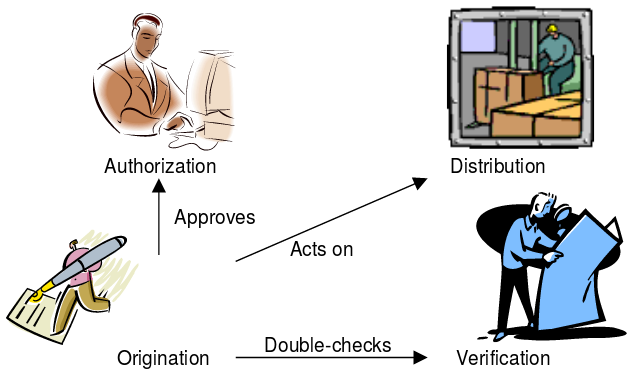
\includegraphics[scale=0.425]{segregation}
 \caption{Una corretta applicazione della \textbf{segregation of duties} con 
quattro componenti.}
\end{figure}


\paragraph*{Controlli compensativi}

Questi tipi di controlli compensano l'assenza di alcuni controlli che possono
essere mancanti o difettosi, o quando la \textit{segregation of duties} non è
possibile. Queste tipologie di controlli sono spesso trasversali.

\subsection{Software per trovare frodi}

Fin dall'inizio del commercio, si iniziò a fare i controlli sui conti. Il
primo tipo di controllo implementato prima dell'arrivo dei computer era la
partita doppia. Ora con il computer sono presenti diversi tipi di software
per trovare delle frodi. Quelli di tipo finanziario vanno per la maggiore.

Il software identifica i vari \textit{outlier}, ovvero tutto ciò che si
comporta diversamente dalla media.

\subsection{Incoraggiare la sicurezza nei dipartimenti IT}

Alcuni punti focali:
\begin{itemize}
  \item Sicurezza fisica
  \item \textit{Segregation of duties} \\
  Una cosa importante da non sbagliare è di mettere i controlli di monitoring
  sullo stesso hardware in cui si ha il software in produzione.
  \item Monitor dei dipendenti
  \item Audit a sorpresa
  \item Rotazione dei lavori
  \item Analisi della documentazione
\end{itemize}

\paragraph*{PO Box} \todo{era riferito a cosa?}

È quello che si definisce un fermo posta, viene dato dall'ufficio postale
presentandosi con un documento d'identità. Il fermo posta non è associato a un
indirizzo di un'abitazione.

\subsection{Esercizi}

Gli esercizi su questa parte sono presenti nella rispettiva sezione
(\ref{EsFrodi2}).

\section{Social Engineering}
		
Oggi è più facile eseguire un \textit{escalation} di privilegi dall'interno,
piuttosto che tentare di entrare nel sistema in maniera non autorizzata.

Un tipico esempio sono le e-mail con degli eseguibili allegati.

Tipici esempi sono:
\begin{itemize}
  \item Le prime 500 persone a registrarsi a questo sito web vinceranno dei
  biglietti.
  \item Il tuo account è stato bloccato, per favore ri-esegui il login.
  \item Fingersi un tecnico IT\footnote{Richiede tempo ma permette di
introdursi all'interno dell'azienda. Il veicolo
di questo attacco è la fiducia.}.
\end{itemize}

\paragraph*{Definizione} Il \textit{social engineering} è convincere le persone
a fare cose che solitamente non farebbero.

\subsection{Come combattere il Social Engineering}

È importante essere aderenti alle procedure di verifica, che possono essere:
\begin{itemize}
  \item Verificare sempre che l'indirizzo e-mail sia dell'azienda.
  \item Verificare che il richiedente sia un impiegato e che ricopra
  effettivamente quel ruolo.
  \item Verificare l'autorizzazione richiesta.
  \item Verificare i record delle transazioni.
\end{itemize}

Anche a livello organizzativo è necessario applicare delle verifiche, che
potrebbero essere:
\begin{itemize}
  \item Classificazione dei dati e definizione del loro trattamento
  \item \textit{Policies} definite per il comportamento degli impiegati
  \item Addestramento dei dipendenti riguardo ai ruoli e alle \textit{policies}
che devono essere applicate
\end{itemize}

\subsection{Statistiche su questo tipo di frodi}

I medicinali contraffatti sono quelli che rendono di più. In generale, la merce
contraffatta è un grosso problema.

Anche il furto d'identità costituisce una grossa frode, soprattutto negli
Stati Uniti.

\section{Esercizi riassuntivi}

Gli esercizi riassuntivi su tutto il capitolo possono essere trovati nella
sezione apposita (\ref{EsFrodi3}).

\chapter{Business Continuity and Disaster Recovery}
\label{BCDR}

Prendiamo ad esempio una delle seguenti aziende:
\begin{itemize}
  \item 1 milioni di account, carte di credito, prestiti
  \item Società di Airline, con 250 voli giornalieri
  \item Farmacia con 5 milioni di prescrizioni all'anno
  \item Fabbrica con 200 impiegati che producono 200,000 prodotti
\end{itemize}

Che cosa succede quando avviene un fallimento di sistema, come una interruzione
di corrente prolungata o un fallimento di server?

\section{Primo passo: Business Impact Analysis}

È di fondamentale importanza analizzare l'impatto che un evento può avere sulla
società. Per capire questo, bisogna porsi la seguente domanda: qual è il
processo più critico dell'azienda?

Non è semplice rispondere a questa domanda, ma è necessario riuscire a
individuarlo.

È anche importante essere in grado di eseguire un'\textbf{analisi dei rischi},
da quelli più piccoli a quelli più grandi\footnote{Un meteorite, ad esempio}. È
anche doveroso chiedersi, come potrebbero questi eventi impattare sull'azienda?
Come si relazionano la safety e la security con questi rischi? E, infine,
quanto tempo impiego per recuperare ciò che ho perso? È possibile ritornare a
lavoro con due modalità:
\begin{enumerate}
  \item In modalità degradata
  \item Ritorno a lavoro a pieno regime
\end{enumerate}

È da tenere conto che più velocemente si vuole tornare ad un regime di lavoro
normale più il costo aumenta.
